\documentclass[11pt,a4paper]{article}
\usepackage[margin=2.3cm]{geometry}
\usepackage[T1]{fontenc}
\usepackage{lmodern}
\usepackage{graphicx}
\usepackage{xcolor}
\usepackage{fancyvrb}
\usepackage{booktabs}
\usepackage{enumitem}
\usepackage[colorlinks=true,linkcolor=teal!60!black,urlcolor=teal!60!black]{hyperref}

\definecolor{teal}{RGB}{0,128,128}
\DefineVerbatimEnvironment{cmd}{Verbatim}{fontsize=\small,frame=single,rulecolor=\color{gray!60},framesep=2mm}
\newcommand{\file}[1]{\texttt{#1}}
\setlength{\parindent}{0pt}
\setlength{\parskip}{0.6em}
\setlist{itemsep=0.2em,topsep=0.3em}

\title{\textbf{PDBsum1 --- User Manual}\\[0.3em]\large Structural summaries of protein--ligand and protein--protein structures,\\run locally with Docker}
\author{PFG Lab}
\date{September 2026}

\begin{document}
\maketitle

\section{What is PDBsum1?}
PDBsum1 is a standalone version of the PDBsum ``Generate'' service. Give it a PDB file --- a crystal structure, a docking result, a model --- and it builds a set of linked web pages that summarise the structure at a glance:
\begin{itemize}
  \item the molecules present (protein chains, DNA/RNA, ligands, metal ions, waters) and their secondary structure;
  \item Ramachandran plot and other quality checks (PROCHECK);
  \item \textbf{ligand pages}, with the LIGPLOT schematic of every hydrogen bond and hydrophobic contact between ligand and protein;
  \item \textbf{protein--protein interface pages} (contacts, hydrogen bonds, salt bridges);
  \item surface \textbf{clefts} (possible binding pockets);
  \item domain diagrams (Pfam) when the file names a UniProt entry.
\end{itemize}
Because it runs on your own machine, your unpublished structures and models never leave the lab.

\begin{figure}[h]
\centering
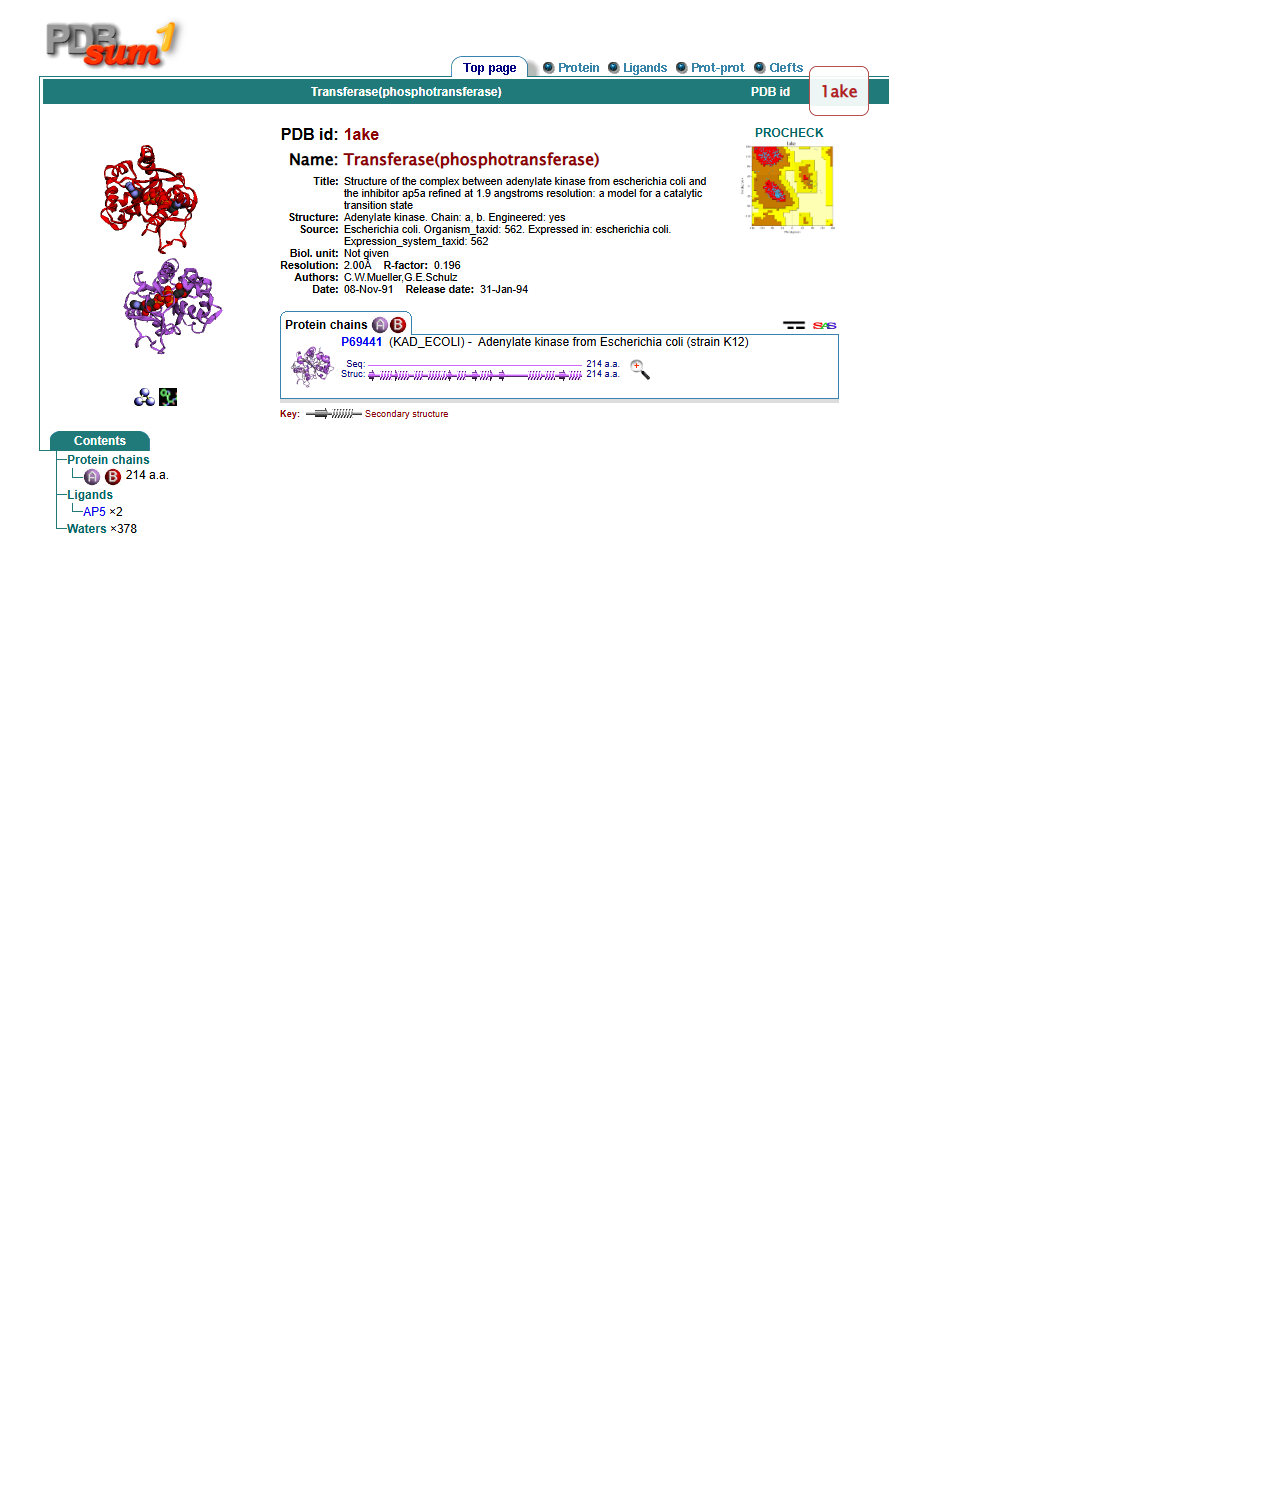
\includegraphics[width=0.78\textwidth,trim=30pt 940pt 380pt 0pt,clip]{figures/overview.png}
\caption{The top page for an example structure (PDB \texttt{1ake}, adenylate kinase with an AP5 inhibitor). The tabs across the top lead to the Protein, Ligands, Prot-prot and Clefts pages.}
\end{figure}

\section{What you need}
PDBsum1 is packaged as a Docker container, so you do \emph{not} install PyMOL, ImageMagick, Ghostscript or anything else yourself. You need:
\begin{itemize}
  \item \textbf{Docker} --- Docker Desktop on Windows/macOS, or Docker Engine on Linux;
  \item an \textbf{internet connection} the first time (to build the image) and whenever you run a structure that names a UniProt entry (used to fetch the domain diagram);
  \item about \textbf{4~GB} of free disk for the image, plus roughly 75~MB of results per structure.
\end{itemize}
If you use the lab server instead (Section~\ref{sec:server}), you need none of this --- only access to the server.

\section{Getting it running on your own computer}
\subsection{One-time setup}
\begin{cmd}
git clone https://github.com/PFG-Lab/PDBsum1.git
cd PDBsum1
docker build -t pfglab/pdbsum1:latest .
\end{cmd}
The build downloads the current wwPDB Chemical Component Dictionary (about 500~MB) and takes a few minutes. You only do this once.

Check that it works:
\begin{cmd}
docker run --rm pfglab/pdbsum1:latest -help
\end{cmd}
You should see the ``Usage is\ldots'' message.

\subsection{Folder layout}
The launcher scripts use two folders next to them:
\begin{center}
\begin{tabular}{ll}
\toprule
\file{input/} & put your PDB files here\\
\file{results/} & PDBsum1 writes its web pages here\\
\bottomrule
\end{tabular}
\end{center}
Both are created automatically the first time you run.

\section{Running PDBsum1}
\subsection{A single structure}
\textbf{Linux / macOS} (in a terminal, inside the \file{PDBsum1} folder):
\begin{cmd}
./pdbsum1.sh myprotein.pdb
\end{cmd}
\textbf{Windows} (in PowerShell, with Docker Desktop running):
\begin{cmd}
.\pdbsum1.ps1 myprotein.pdb
\end{cmd}
You can give the path to a file anywhere on your computer; it is copied into \file{input/} for you. A typical two-chain structure with one ligand takes under a minute.

When it finishes, open \textbf{\file{results/index.html}} in any web browser.

\subsection{Choosing the PDB code}
Every run is filed under a 4-character \emph{PDB code}. The launcher picks it like this:
\begin{itemize}
  \item a file called \file{pdbXXXX.ent} or \file{pdbXXXX.pdb} uses \texttt{XXXX};
  \item a file whose name is exactly four letters/digits, such as \file{1ake.pdb}, uses that name;
  \item otherwise PDBsum1 numbers the runs \texttt{a001}, \texttt{a002}, \ldots
\end{itemize}
To choose your own code, add it after the file name:
\begin{cmd}
./pdbsum1.sh docking_run7_best.pdb r7b1
\end{cmd}
Using your own codes is worthwhile when you process many models, because the run list on the front page then makes sense at a glance.

\subsection{Many structures at once}
Put all the PDB files in \file{input/}, and make a plain text file (for example \file{input/list.txt}) with one file name per line, optionally followed by a code:
\begin{cmd}
modelA.pdb  mdlA
modelB.pdb  mdlB
1ake.pdb
\end{cmd}
Then run:
\begin{cmd}
./pdbsum1.sh -l list.txt
\end{cmd}
The front page (\file{results/index.html}) lists every structure processed.

\subsection{Options}
\begin{center}
\begin{tabular}{lp{10cm}}
\toprule
\file{-nomaxchn} & Calculate clefts even for structures with more than four protein chains. \textbf{Warning:} this can take very long for large assemblies.\\
\file{-help} & Show the usage message.\\
\bottomrule
\end{tabular}
\end{center}
(Links in the results are always made relative, so you can move or zip the \file{results} folder and it will still work.)

\section{Preparing your PDB file}
PDBsum1 repairs some common problems (missing chain identifiers, duplicate atom names), but you will get the best results if the file:
\begin{itemize}
  \item is in standard PDB format (docking and modelling programs sometimes are not --- if a run fails, check this first);
  \item has a \textbf{TITLE} record. The title appears on the results page and helps you tell structures apart;
  \item has a \textbf{DBREF} record naming the UniProt accession of each chain. With it, PDBsum1 downloads the Pfam domains and draws the domain diagram. Without it, everything else still works.
\end{itemize}
Example \texttt{DBREF} line for adenylate kinase:
\begin{cmd}
DBREF  1AKE A    1   214  UNP    P69441   KAD_ECOLI        1    214
\end{cmd}
Ligands are recognised by their three-letter residue name (for example \texttt{AP5}) and drawn using the wwPDB Chemical Component Dictionary. A custom ligand with an unusual name is still listed and analysed, but its LIGPLOT diagram may be less complete.

\section{Reading the results}
Open \file{results/index.html}, then click your structure. Every page has the same tabs across the top.

\begin{description}[style=nextline]
  \item[Top page] Title, source organism, resolution, a thumbnail of the fold, the secondary-structure cartoon per chain, the PROCHECK Ramachandran thumbnail, and a contents tree on the left.
  \item[Protein] Per-chain pages: sequence and secondary structure, Ramachandran plot, motifs (helices, strands, $\beta$-turns, hairpins, disulphide bridges).
  \item[Ligands] One page per ligand or metal: 2D and 3D depiction and the \textbf{LIGPLOT} diagram of its contacts with the protein (Figure~\ref{fig:lig}). Green dashed lines are hydrogen bonds with their distances; red spokes are hydrophobic contacts. PostScript and PDF versions are provided for figures and papers.
  \item[Prot-prot] For complexes: the contacting chains, interface residues, hydrogen bonds, salt bridges and non-bonded contacts.
  \item[Clefts] The largest surface pockets, ranked by volume --- useful for spotting a binding site.
\end{description}

\begin{figure}[h]
\centering
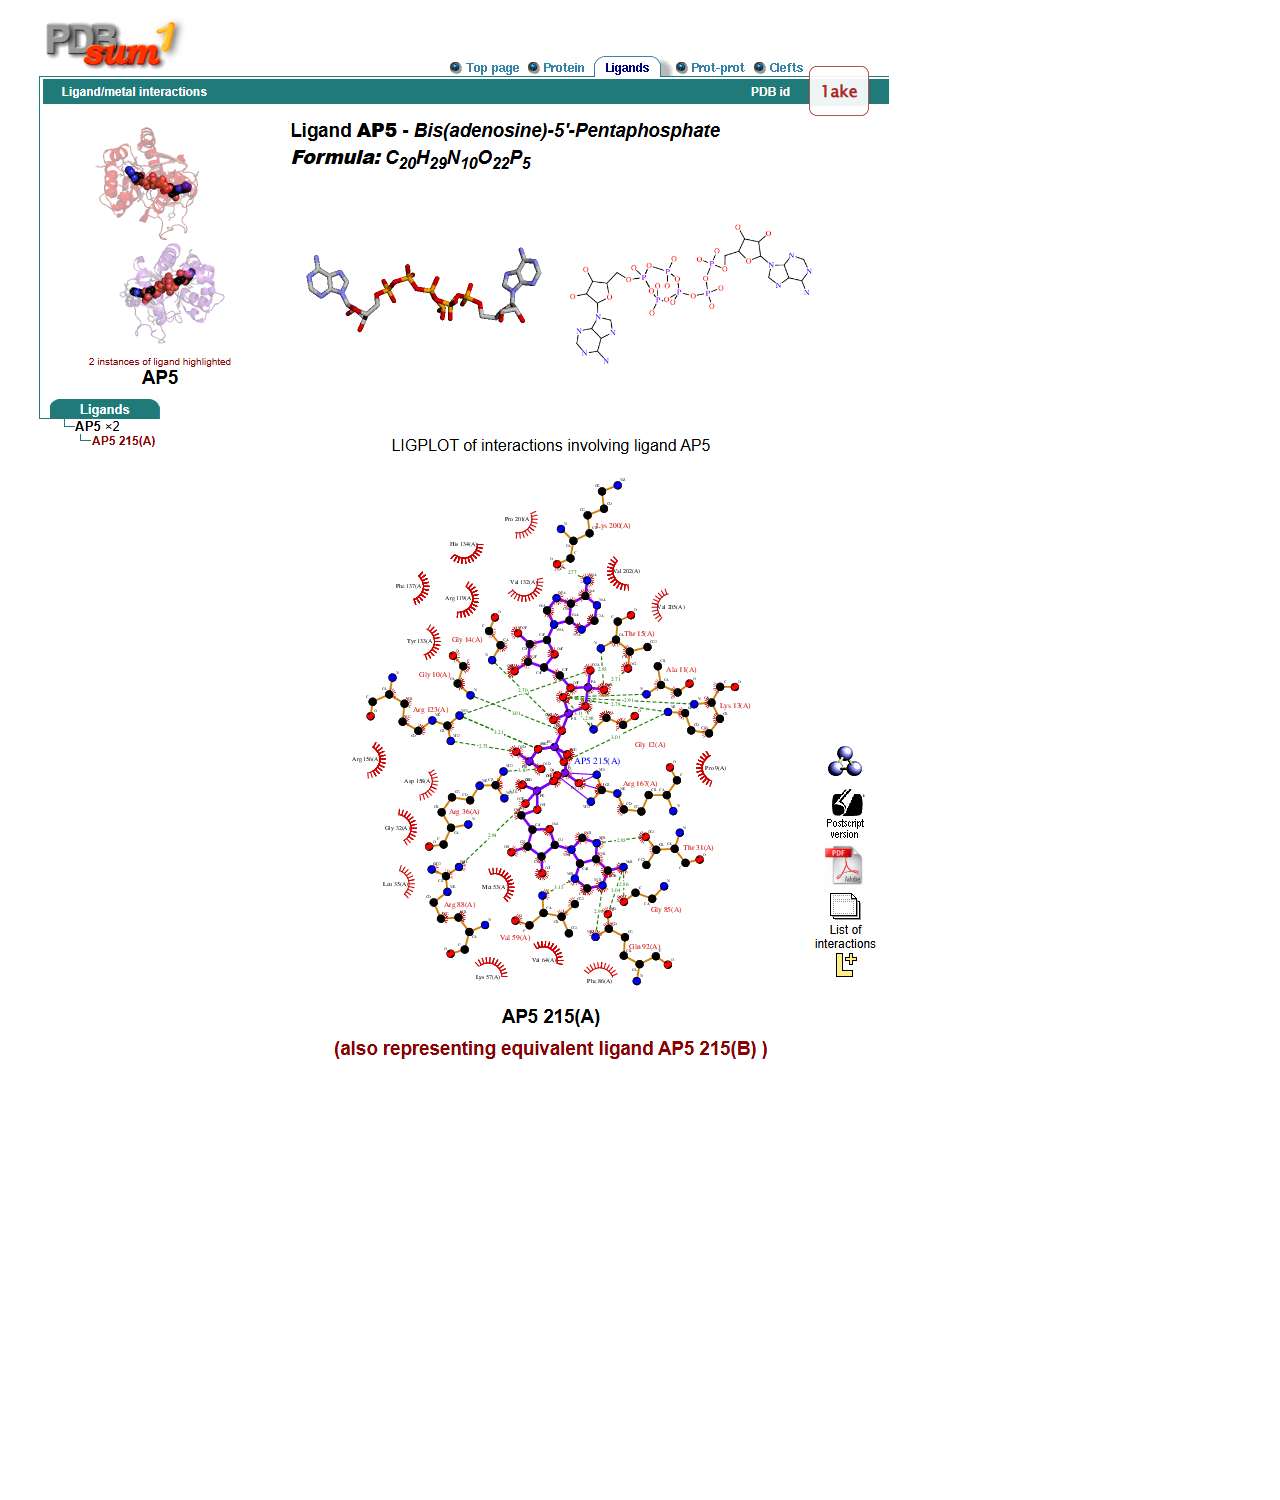
\includegraphics[width=0.78\textwidth,trim=30pt 425pt 380pt 0pt,clip]{figures/ligand.png}
\caption{The Ligands page: chemical structure of AP5 and its LIGPLOT interaction diagram.}
\label{fig:lig}
\end{figure}

\subsection{What is in the results folder}
\begin{center}
\begin{tabular}{lp{10cm}}
\toprule
\file{index.html} & Front page: list of the structures you processed.\\
\file{runs/} & The list of all runs so far.\\
\file{docs/} & The built-in help pages (opened from the ``help'' icons).\\
\texttt{xx/CODE/} & One folder per structure (the folder is named from the middle two characters of the code, e.g.\ \file{ak/1ake}). Inside: \file{html/} (the pages), images (\file{gif/}, \file{ligplot/}, \file{pymol/}, \ldots) and the cleaned coordinates.\\
\bottomrule
\end{tabular}
\end{center}
\textbf{To share results with a colleague}, zip the whole \file{results} folder; they open \file{index.html} in a browser --- nothing needs to be installed on their side.

\textbf{3D viewing.} The small PyMOL and RasMol icons on the pages generate scripts for those programs; they only work if you have them installed on your own computer. The images already on the pages do not need them.

\section{Using the lab server}\label{sec:server}
PDBsum1 is installed on the lab's server at \file{/mnt/bilal/pdbsum1}, kept on the large data disk so the operating system disk is not affected. Ask Dr.~Bilal for access. Then, on the server:
\begin{cmd}
cd /mnt/bilal/pdbsum1
cp /path/to/myprotein.pdb input/
./pdbsum1.sh myprotein.pdb
\end{cmd}
Results appear in \file{/mnt/bilal/pdbsum1/results}. Copy the folder to your own computer (for example with \texttt{scp -r} or a file-transfer program) and open \file{index.html} in your browser. For a long batch, start it inside \texttt{tmux} so that it keeps running if your connection drops:
\begin{cmd}
tmux new -s pdbsum1
./pdbsum1.sh -l list.txt
# detach with Ctrl-b then d; reattach later with: tmux attach -t pdbsum1
\end{cmd}

\section{Troubleshooting}
\begin{description}[style=nextline]
  \item[``Cannot connect to the Docker daemon'' / nothing happens] Docker is not running. Start Docker Desktop (Windows/macOS) or the Docker service (Linux) and try again.
  \item[The run seems stuck] A normal run prints progress lines (``Running \ldots'') and the number of files in \file{results/} keeps growing. If neither changes for several minutes, stop it (Ctrl-C) and check the input file. Very large assemblies with clefts switched on are the usual reason for a genuinely long run.
  \item[The run finishes but a page is missing or empty] The PDB file probably has format problems. Open the run's \file{logs/} folder (inside its results folder) and read the log for the step that failed.
  \item[No domain (Pfam) diagram] The file has no \texttt{DBREF} record, or the computer could not reach the UniProt/InterPro web services.
  \item[Permission problems on Linux] Use the \file{pdbsum1.sh} launcher --- it runs the container as your own user, so the results belong to you. Results created by running \texttt{docker run} by hand are owned by \texttt{root}.
  \item[Something else] Send the contents of the run's \file{logs/} folder and the input file to the lab's IT contact.
\end{description}

\section{Notes for the maintainer}
\begin{itemize}
  \item This repository is a fork of \url{https://github.com/RomanLas/PDBsum1}. The upstream files are unchanged; the Docker setup is added on top (\file{Dockerfile}, \file{docker/}, \file{pdbsum1.sh}, \file{pdbsum1.ps1}, \file{docker-compose.yml}, this manual), so upstream updates can be merged cleanly.
  \item \textbf{Upstream bug worked around.} The upstream \texttt{hbadd} program crashes (segmentation fault) when given the full, current wwPDB \file{components.cif}. The image therefore wraps it (\file{docker/hbadd-wrapper.sh}): \texttt{hbadd} is handed a trimmed dictionary containing only the residue types that occur in the structure being processed. The other programs read the full dictionary unchanged.
  \item PDBsum1 needs a virtual display for PyMOL; the entrypoint starts one (\texttt{Xvfb}). Docker's standard \texttt{xvfb-run} helper hangs when it is the container's first process, which is why it is not used.
  \item The upstream repository carries no licence file. Check the terms with the authors before redistributing the image outside the lab.
  \item Refresh the chemical dictionary by rebuilding the image (\texttt{docker build --no-cache}).
\end{itemize}

\section{Credits and citation}
PDBsum and PDBsum1 are the work of Roman Laskowski and colleagues (EMBL-EBI). If you use PDBsum in a publication, please cite the PDBsum paper (Laskowski RA, Jab{\l}o{\'n}ska J, Pravda L, Va{\v r}ekov{\'a} RS, Thornton JM. PDBsum: Structural summaries of PDB entries. \emph{Protein Science} 2018;27:129--134) and check the PDBsum1 pages for any updated citation guidance. For installation problems with the underlying software, see the contact given in the upstream installation notes.

\end{document}
